\documentclass{article}

\usepackage[final]{dip_2021}

\usepackage[utf8]{inputenc} % allow utf-8 input
\usepackage[T1]{fontenc}    % use 8-bit T1 fonts
\usepackage{hyperref}       % hyperlinks
\usepackage{url}            % simple URL typesetting
\usepackage{booktabs}       % professional-quality tables
\usepackage{amsfonts}       % blackboard math symbols
\usepackage{nicefrac}       % compact symbols for 1/2, etc.
\usepackage{microtype}      % microtypography
\usepackage{CJKutf8}        % Chinese word
\usepackage{graphicx}       % Graphs/Figures
\usepackage{amsmath}
\setcitestyle{square}
\usepackage{caption}
\usepackage{subcaption}
\usepackage{soul}
\usepackage{color, xcolor}

%\usepackage{natbib}         % natbib package for citation
%\usepackage[square]{natbib}

%\graphicspath{{imgs/}}

\title{DIP Final Project: Depth Image Inpainting}

\author{%
  Li-Wei Fu\\
  r10942078\\
  Graduate Institute of Communication Engineering\\
  National Taiwan University\\
  \texttt{r10942078@ntu.edu.tw} \\
  \And
  Po-Yen Tseng \\
  r09521504\\
  Graduate Institute of Civil Engineering\\
  National Taiwan University \\
  \texttt{r09521504@ntu.edu.tw}\\ 
  \And
  Yu-Kai Ling \\
  r09921054 \\
  Graduate Institute of Electrical Engineering\\
  National Taiwan University\\
  \texttt{r09921054@ntu.edu.tw} \\
  \And
  Wei-Min Chu\\
  r10546017\\
  Graduate Institute of Industrial Engineering\\
  National Taiwan University\\
  \texttt{r10546017@ntu.edu.tw} \\
}

\begin{document}
\begin{CJK*}{UTF8}{bkai}
\maketitle

\renewcommand{\baselinestretch}{1.50}\normalsize
\section{Introduction}
Image inpainting\cite{inpainting}對於電腦視覺與影像處理來說是一個非常重要的研究領域,我們的主題focus在depth image inpainting,深度照相機拍攝出來的圖片都會有一些缺失的pixels,原因通常是拍到有反光還有透明的物體,或是距離深度已超出相機能偵測到的距離上限,此時相機就無法得到深度資訊。

\begin{figure}[h]
    \centering
    \begin{subfigure}[h]{0.45\textwidth}
        \centering
        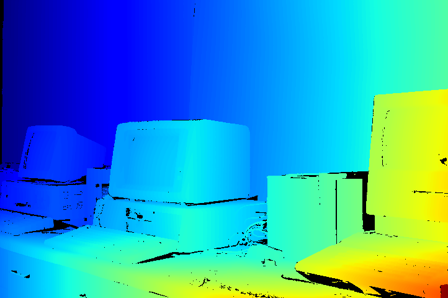
\includegraphics[width=0.9\textwidth]{imgs/image_inpaint.png}
        \caption{Before inpainting}
        \label{fig:image_inpainting_a}
    \end{subfigure}
    \begin{subfigure}[h]{0.45\textwidth}
        \centering
        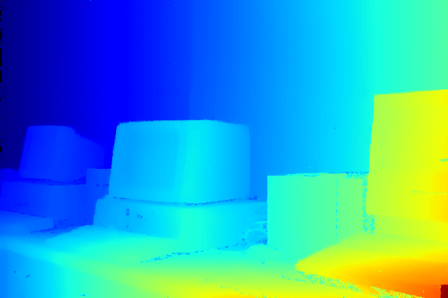
\includegraphics[width=0.9\textwidth]{imgs/image_inpaint2.png}
        \caption{After inpainting}
    \label{fig:image_inpainting_b}
    \end{subfigure}
    \caption{Example of depth image inpainting}
    \label{fig:image_inpainting}
\end{figure}



在本次作業我們研究了幾篇使用傳統image processing方法的論文,方法都是把depth image inpainting轉換成一個Matrix Completion的問題,基於low rank、low gradients等統計學上的假設,設計一些目標函數和constrain,使用ADMM等演算法來解這些convex optimization problems。


我們主要參考Depth Image Inpainting:
Improving Low Rank Matrix Completion with
Low Gradient Regularization \cite{lrl0phi}這篇paper的方式,花了很多時間用python重現論文的貢獻 {$\mathrm{LRL0^{\psi}}$},同時也使用python重現了LR\cite{LR}、LRTV\cite{LRTV}、LRL0\cite{LRl0}這三篇paper的方法,驗證論文的結果,並且發現這些方法對於太大的hole無法完全的填補。因此,我們嘗試運用本堂課程在morphology章節所學到的知識,加上histogram analysis,來將較大的洞做填補,進一步提升$\mathrm{LRL0^{\psi}}$的填補效果,得到一個完全沒有缺失值、最好的結果。


我們提出的填補方法簡單、很適合套用在中型大小的hole,且運算速度極快,結合前述paper的傳統方法可以達到real time,這是目前deep learning method也無法達到的。我們所有的實作都整理在 \href{https://github.com/kai860115/DIP-FinalProject}{GitHub(https://github.com/kai860115/DIP-FinalProject)} 上,如果有需要的話可以參考。


\section{Methodology \& Implementation Details}

\subsection{Paper survey}
目前在Depth image inpainting領域效果最好的model是Deep Depth Completion of a Single RGB-D Image \cite{singledepth}的方法,這篇論文被引用多次,且方法好懂,利用一張圖片的表面法向量與遮擋邊界來作為input的 feature,使用深度學習的模型來填補一張圖片的深度資訊,然而因為此方法較為耗時、需要大量的GPU運算資源訓練深度學習的model來進行預測,而且與本堂課程較無關係,因此我們捨棄了此篇論文的做法。

接者我們打算使用Fast Generation of High Fidelity RGB-D Images 
Deep-Learning with Adaptive Convolution \cite{fast}這篇論文的做法,速度為前一篇的10倍以上,在深度學習網路的Convolution 層前加入了傳統image processing 的作法,並架設refinement network來進一步的微調,然而因為此篇paper的pretrained model 與原paper所提供的有所不同,在reproduce過程有困難,我們最後沒有使用此篇paper。

\begin{figure}[h]
\centering
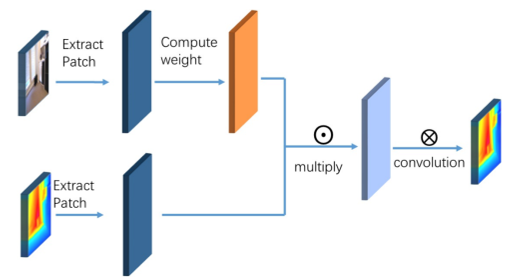
\includegraphics[width=0.9\textwidth]{imgs/refinement.png}
\caption{Refinement Network}
\label{fig:refinement_network}
\end{figure}



在paper survey的過程中,我們發現很多傳統的方法會把depth image inpainting轉換成一個Matrix Completion的問題,圖片上的缺失值可以運用matrix completion algorithms來做到image inpaiting的效果,且在這幾篇論文中我們發現深度的圖片通常都具有較低的gradients,gradients 在部份地方會有vanish的現象,跟它的深度也許有相對應的關係,我們最後便往Matrix Completion跟low gradients的關鍵字做查找,並使用Depth Image Inpainting:
Improving Low Rank Matrix Completion with
Low Gradient Regularization\cite{lrl0phi}這篇paper作為我們final project主要實作的paper。


\subsection{Background}
此篇論文的核心概念便是用到Low rank的假設作為基礎,我們可以把圖片當成是一個Matrix,而圖片的hole(黑色的部分)為需要填補的缺失值,只要rank遠小於matrix的長寬m跟n,那缺失的entries就有可能可以被recover回來。



而這篇paper具體的填補方法,便是採用Low-rank low gradient approach,此方法為Low gradient regularization加上Low-rank assumption並進行微調,作者將這個方法取名為$\mathrm{LRL0^{\psi}}$,在介紹此方法之前,先來講解此篇paper的另外兩個比較的方法,Low rank total variation (LRTV) \cite{LRTV}與Low rank L0 gradient (LRL0) \cite{LRl0}。

\subsubsection{The low rank total variation (LRTV)}
一般的Matrix Completion algorithms在針對low rank的image recovery上會有一個重要的限制,因為當hole過大時,有時會發生整個row或是整個column都是缺失值的情形,在演算法上便無法填補這些缺失值,而Low-rank and total variation regularization 便是為了解決這樣的問題,total variation是將整個圖片進行梯度上的整合,並利用一個函數來對每個pixel上的梯度進行正規化與積分計算,再利用正規化的值進行填補,並設立一個cost function,變成一個最佳化問題,最後利用Alternating Direction Method of Multipliers (ADMM)演算法來進行求解。

\subsubsection{The low rank L0 gradient (LRL0)}
而利用total variation的這個方法雖然可以用來鬆弛L0的gradient,但total variration的這個方法同時也使得gradient較大的地方影響變小,會讓原來圖片的邊緣和邊界受到影響,gradient影響較不明顯,因此LRL0的作法便是採用L0的gradient作為依據,去計算一張圖片gradient為0的部分,看深度的變化幅度,並進行L0 gradient的正規化後,放入最佳化的式子中,設置一個L0 gradient的minimization problem來進行求解。

\subsubsection{The Low rank low gradient approach (LRL0$\mathrm{^{\psi}}$)}
而此篇paper的做法便是將The low rank L0 gradient (LRL0)\cite{LRl0} 進行改良,使用一種低梯度正規化的方式,減少對gradient為1的影響,同時在非零的gradient上面進行懲罰,來讓深度有逐漸的變化,並將low gradient正規化跟low rank的正規化進行結合,來成為depth圖繪製的方式,並將最後結果與上述兩個方法進行比較。


\subsubsection{Peak signal-to-noise ratio (PSNR)}
而 PSNR \cite{psnr}是$\mathrm{LRL0^{\psi}}$這篇論文的主要衡量指標,PSNR是一個比率,用於表示一個信號的最大功率和影響它的破壞性噪點的功率,即為一個影像修復後和原來修復前的影像比質量的好壞,PSNR越高,代表圖片修復後的效果越好,而MSE代表真實的圖像和含有噪點的圖像的所有像素差的平方再取平均值,MSE與PSNR的公式如下:

\begin{equation}
    MSE = \frac{1}{H \times W} \sum^H_{i=1} \sum^W_{j=1} (X(i,j) - Y(i,j))^2
\end{equation}

\begin{equation}
    PSNR = 10 \log_{10} \frac{(2^n-1)^2}{MSE}
\end{equation}

\subsection{Dataset}
Dataset 的部份我們是依據論文使用Middlebury Stereo Dataset,將原始的圖片加入雜訊損壞後,作為修復的目標,如 Figure \ref{fig:example_of_dataset}所示。


\begin{figure}[h]
    \centering
    \begin{subfigure}{0.45\textwidth}
        \centering
        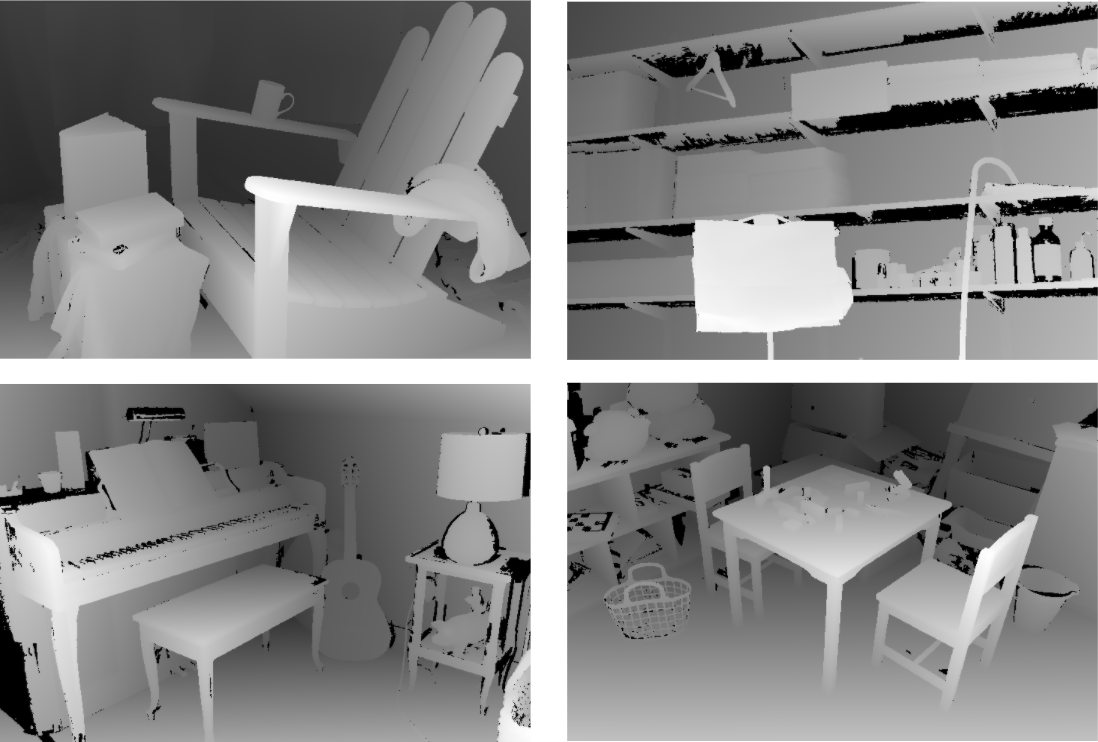
\includegraphics[width=0.9\textwidth]{imgs/dataset1.png}
        \caption{Original}
    \end{subfigure}
    \begin{subfigure}{0.45\textwidth}
        \centering
        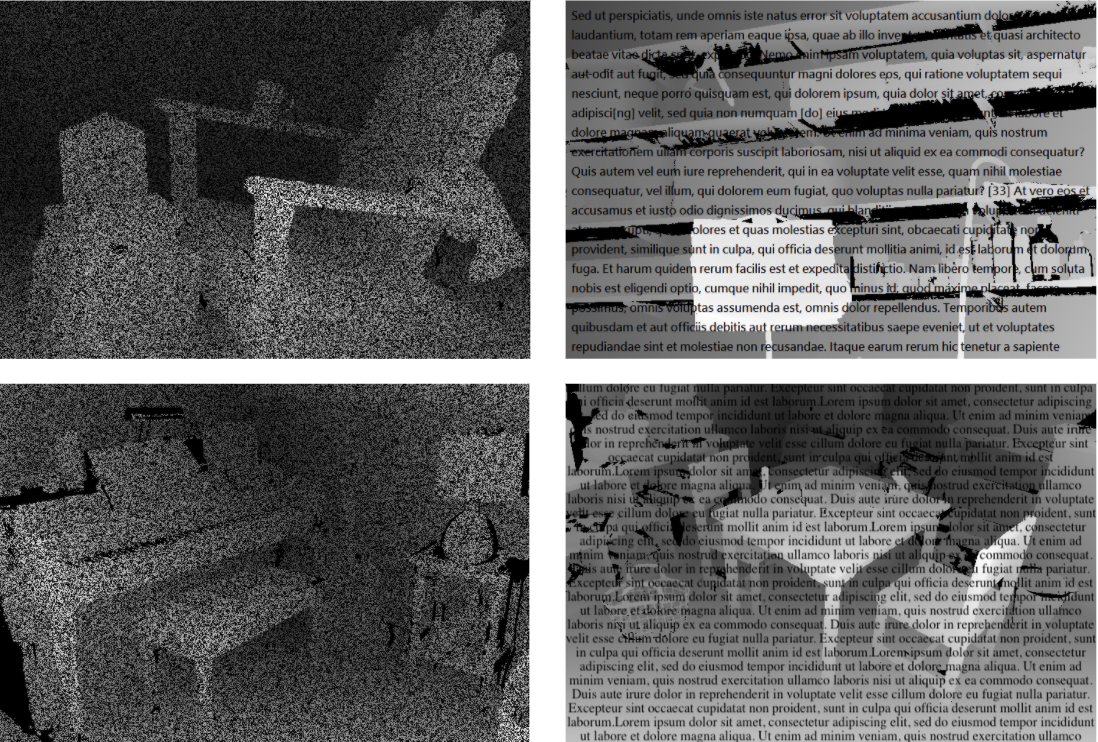
\includegraphics[width=0.9\textwidth]{imgs/dataset2.png}
        \caption{Damaged}
    \end{subfigure}
    \caption{Example of the dataset}
    \label{fig:example_of_dataset}
\end{figure}

\subsection{Reproduce result}
我們用python重現了此篇paper的$\mathrm{LRL0^{\psi}}$方法,結果如 Figure \ref{fig:result_of_lrl0psi} 所示。

\begin{figure}[h]
    \centering
    \begin{subfigure}[h]{0.3\textwidth}
        \centering
        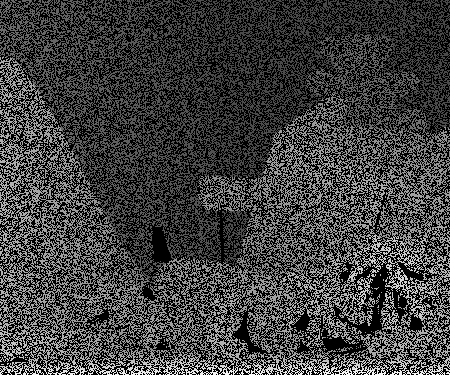
\includegraphics[width=0.9\textwidth]{imgs/Teddy_missing.png}
        \caption{Input image}
        \label{fig:before_lrl0psi}
    \end{subfigure}
    \begin{subfigure}[h]{0.3\textwidth}
        \centering
        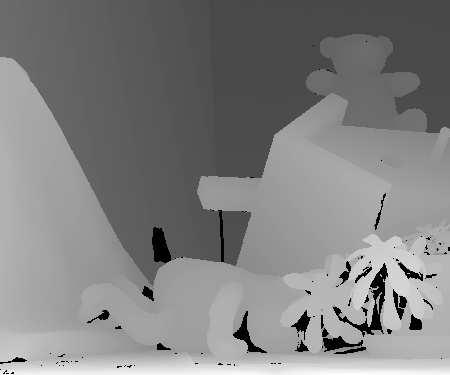
\includegraphics[width=0.9\textwidth]{imgs/Teddy_disp.png}
        \caption{The result of the paper}
    \label{fig:after_lrl0psi}
    \end{subfigure}
    \begin{subfigure}[h]{0.3\textwidth}
        \centering
        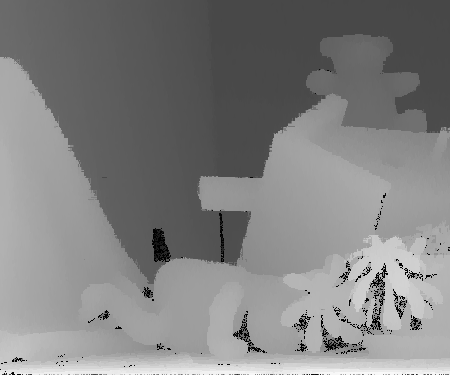
\includegraphics[width=0.9\textwidth]{imgs/Teddy_lrl0phi.png}
        \caption{The result of our implement}
    \label{fig:after_lrl0psi}
    \end{subfigure}
    \caption{The comparison of our implement and the paper}
    \label{fig:result_of_lrl0psi}
\end{figure}


\section{Our Improvement}

如 Figure \ref{fig:result_of_lrl0psi} 所示,我們發現 $\mathrm{LRL0^{\psi}}$ 對於修補破洞有著很好的效果,PSNR 也相當高,但是在對於破洞較大的地方,修補效果不是很理想,於是我們想針對這個部分進行補強。我們使用了上課所提到的方式,先使用影像二值化的方式來找出hole的位置 (Figure \ref{fig:details_of_our_improvement_hole}),接著將hole做不同次數的dilation (Figure \ref{fig:details_of_our_improvement_dilation}),然後用做完dilation的圖片和原始圖片相減,即可得到原本 hole 周圍的 pixels (Figure \ref{fig:details_of_our_improvement_boundary}),我們將 hole 做分群 (Figure \ref{fig:details_of_our_improvement_cluster_hole} 與 Figure \ref{fig:details_of_our_improvement_cluster_boundary}),分析每個 hole 周圍的 pixels 值,
利用 histogram 統計 (Figure \ref{fig:histogram_of_boundary}),將出現機率乘以深度算出期望值填入原本的 hole 中,就會得到結果如 Figure \ref{fig:result_of_our_improvement}。

因為深度圖片具有 low gradient 的特性,pixel value 的變化在小範圍內不會很劇烈,所以在 Figure \ref{fig:histogram_of_boundary} 中我們可以看到 hole 的邊界上的 pixel value 都集中在某幾個值上,也因為這個特性,我們使用 hole 邊界的 pixels 來估計缺失值效果很好。經過實驗,我們的這個方法在直徑 15 pixel 以內的破洞填補效果最好,愈大的洞因為橫跨不同深度的可能性愈高,而修補效果下降。

\begin{figure}[h]
    \centering
    \begin{subfigure}[h]{0.3\textwidth}
        \centering
        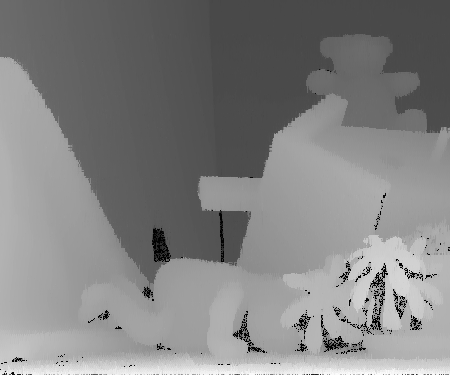
\includegraphics[width=0.9\textwidth]{results/original.png}
        \caption{The result of $\mathrm{LRL0^{\psi}}$}
    \end{subfigure}
    \begin{subfigure}[h]{0.3\textwidth}
        \centering
        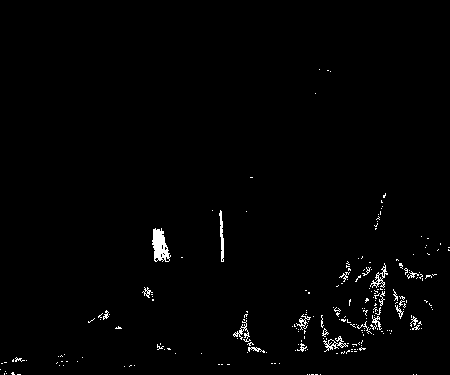
\includegraphics[width=0.9\textwidth]{results/holes.png}
        \caption{The holes}
        \label{fig:details_of_our_improvement_hole}
    \end{subfigure}
    \begin{subfigure}[h]{0.3\textwidth}
        \centering
        
\includegraphics[width=0.9\textwidth]{results/holes_dilated.png}
        \caption{Dilation}
        \label{fig:details_of_our_improvement_dilation}
    \end{subfigure}
    \begin{subfigure}[h]{0.3\textwidth}
        \centering
        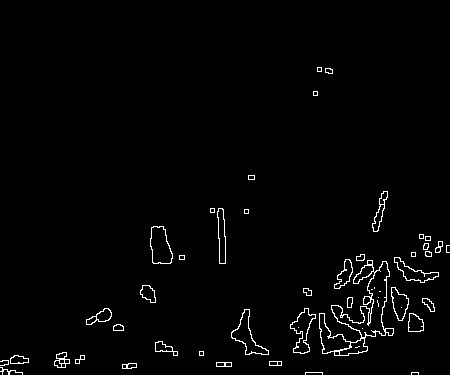
\includegraphics[width=0.9\textwidth]{results/boundries.png}
        \caption{The boundary of the holes}
        \label{fig:details_of_our_improvement_boundary}
    \end{subfigure}
    \begin{subfigure}[h]{0.3\textwidth}
        \centering
        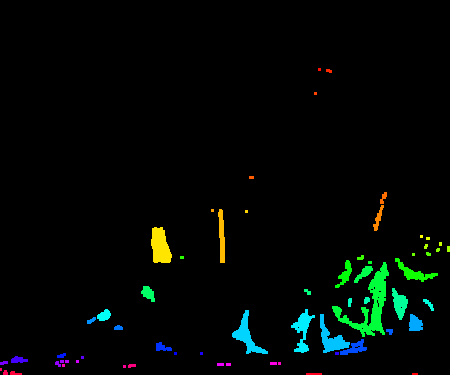
\includegraphics[width=0.9\textwidth]{results/holes_cluster.png}
        \caption{The cluster of the holes}
        \label{fig:details_of_our_improvement_cluster_hole}
    \end{subfigure}
    \begin{subfigure}[h]{0.3\textwidth}
        \centering
        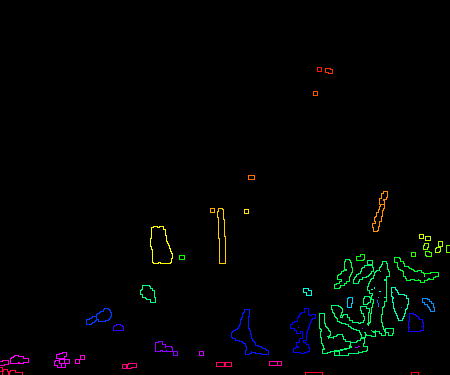
\includegraphics[width=0.9\textwidth]{results/boundries_cluster.png}
        \caption{The cluster of the boundaries}
        \label{fig:details_of_our_improvement_cluster_boundary}
    \end{subfigure}
    \caption{Some details of our improvement}
    \label{fig:details_of_our_improvement}
\end{figure}

\begin{figure}[h]
\centering
    \begin{minipage}{.45\textwidth}
        \centering
        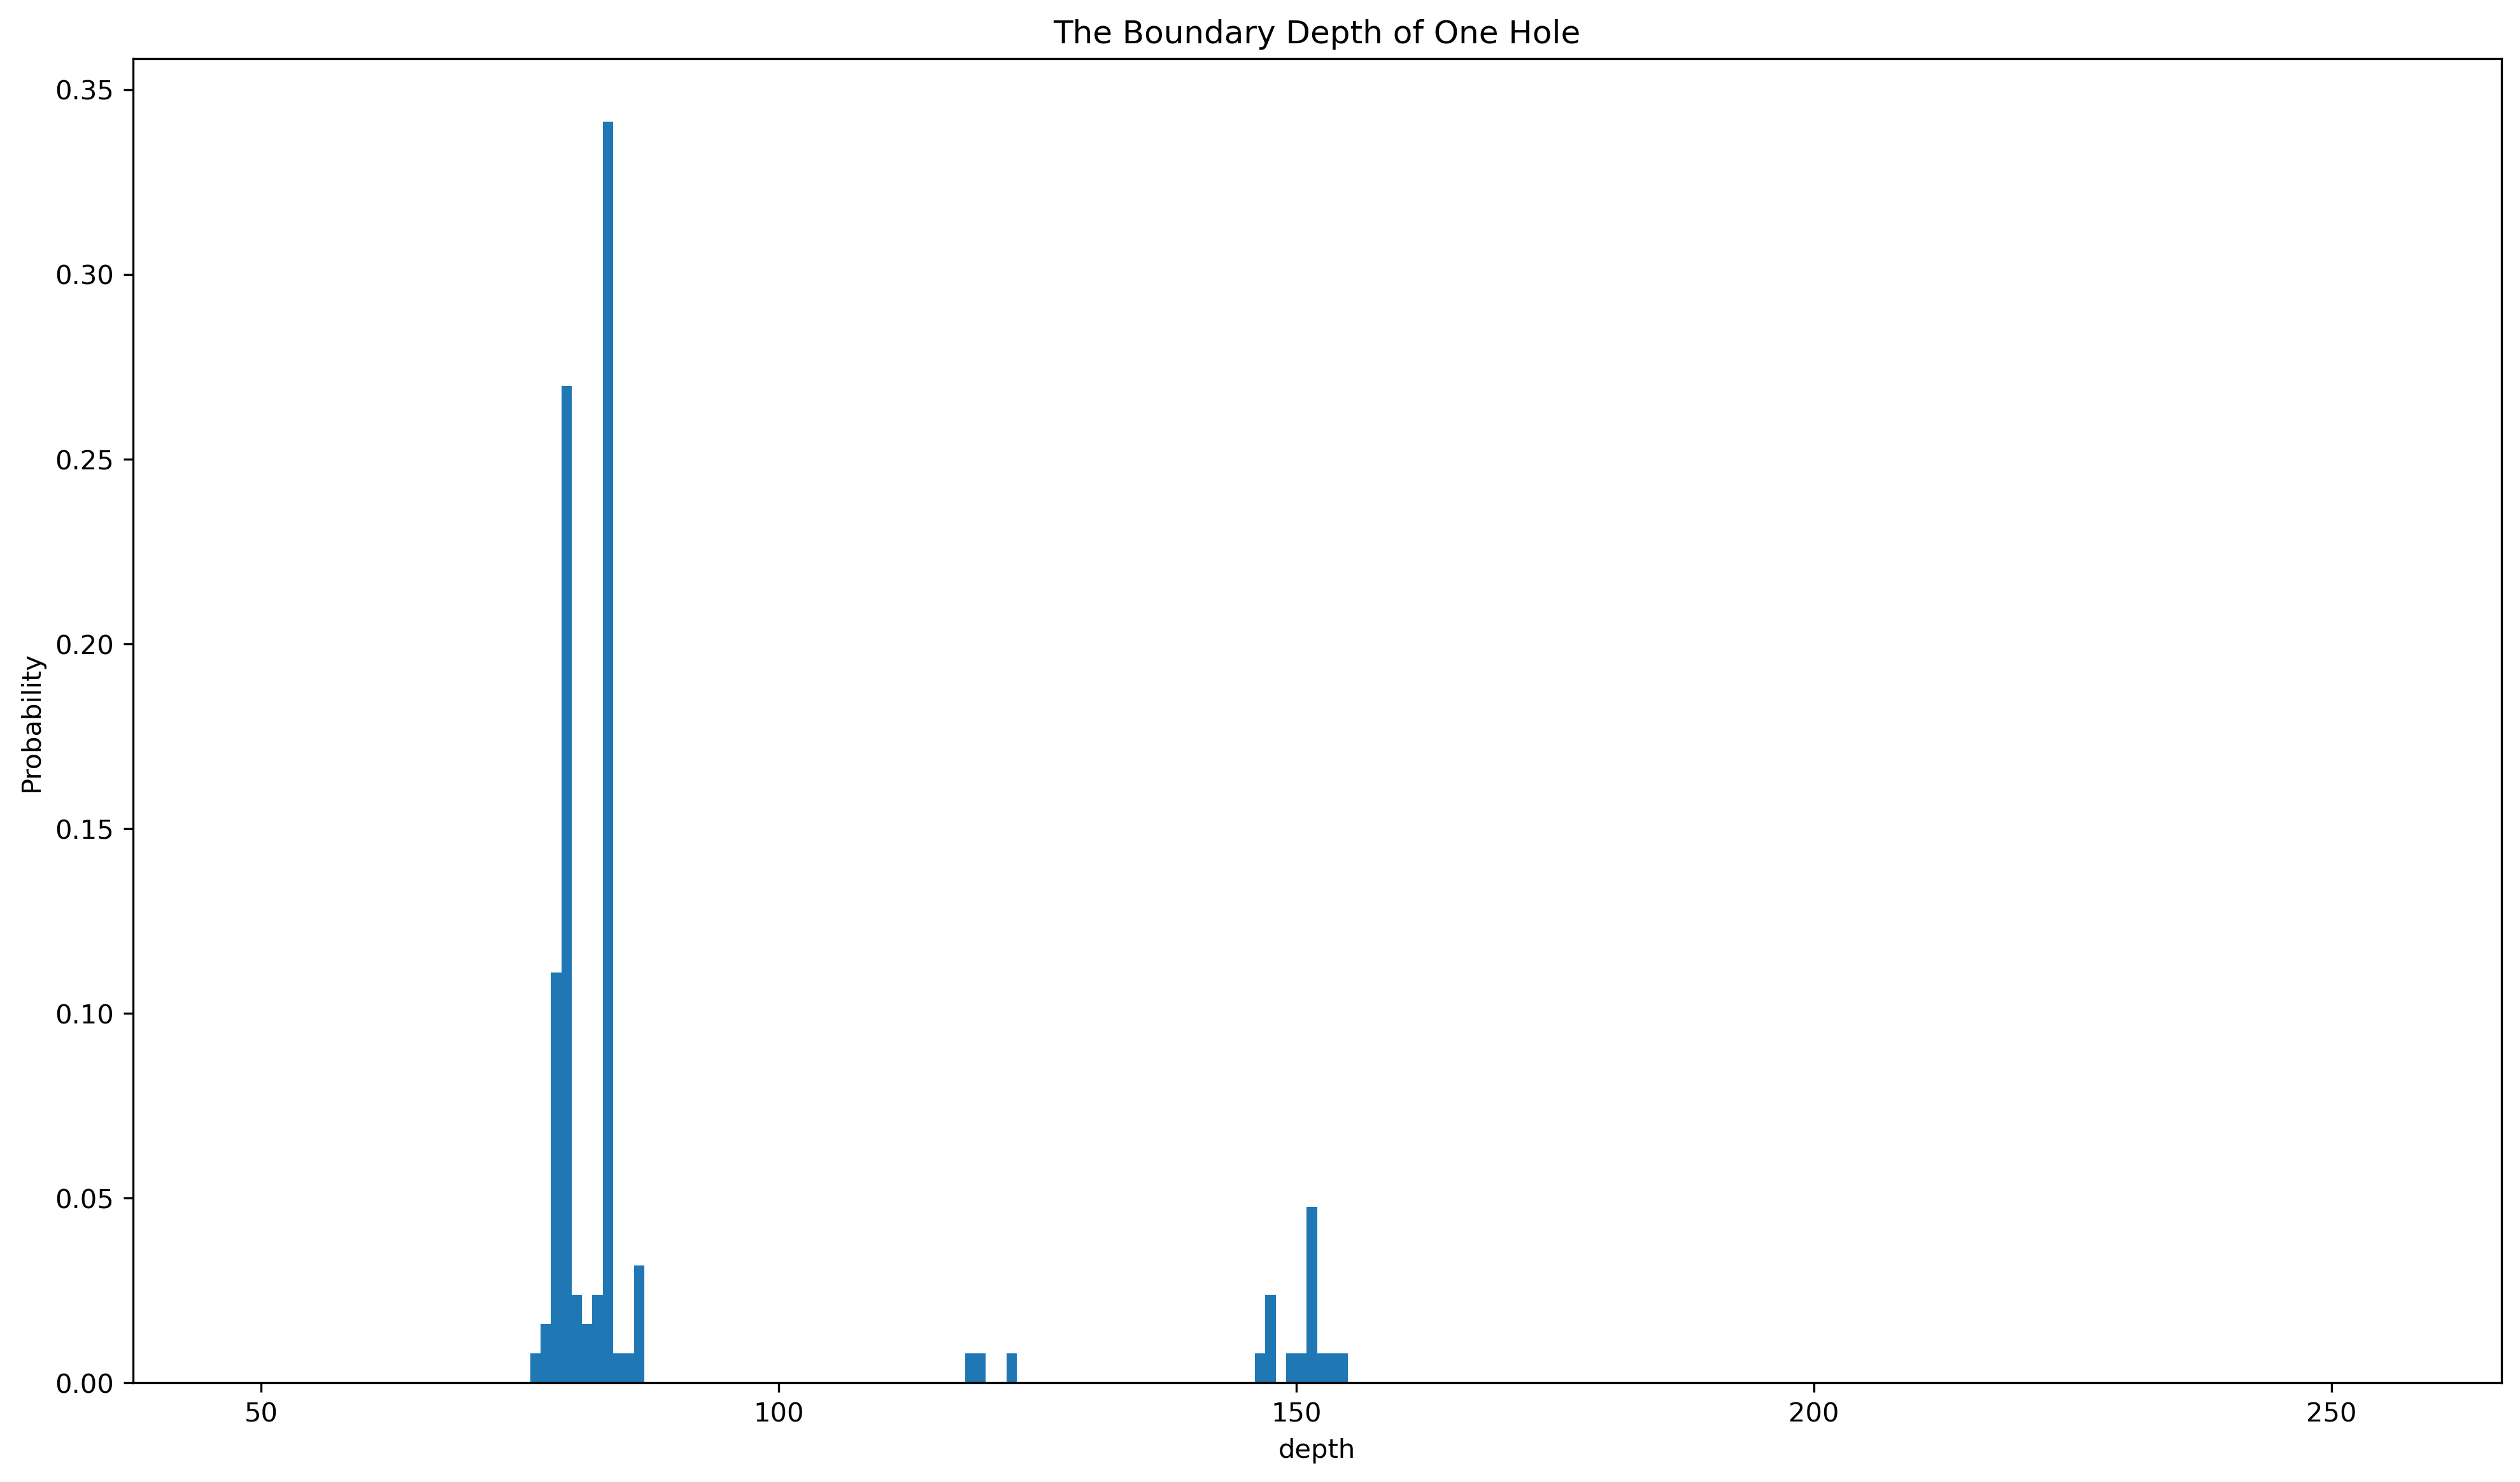
\includegraphics[width=0.9\textwidth]{results/historgram.png}
        \caption{The boundary histogram analysis}
        \label{fig:histogram_of_boundary}
    \end{minipage}
    \begin{minipage}{.45\textwidth}
        \centering
        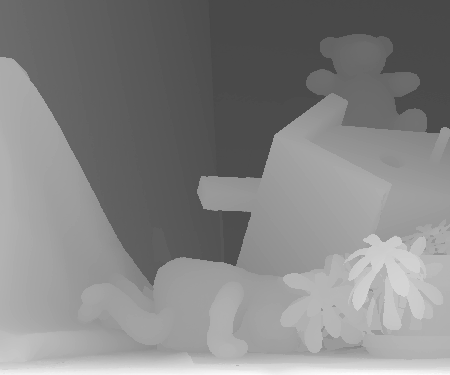
\includegraphics[width=0.64\textwidth]{results/plus.png}
        \caption{The result of our improvement}
        \label{fig:result_of_our_improvement}
    \end{minipage}
\end{figure}


\section{Sensitivity Analysis}

我們針對我們提出的修補方法進行了敏感度分析,希望找出適合的參數來使我們的方法有最好的效果。首先是dilation會使用到的kernel shape比較,我們分別使用正方形、菱形、十字形的kernel在同一張圖片進行測試,kernel示意圖如 Figure \ref{fig:dilation_kernel} 所示。

\begin{figure}[h]
\centering
    \begin{subfigure}{.3\textwidth}
        \centering
        
\includegraphics[width=0.9\textwidth]{imgs/RECT.png}
        \caption{Square}
    \end{subfigure}
    \begin{subfigure}{.3\textwidth}
        \centering
        
\includegraphics[width=0.9\textwidth]{imgs/diamond.png}
        \caption{Diamond}
    \end{subfigure}
    \begin{subfigure}{.3\textwidth}
        \centering
        
\includegraphics[width=0.9\textwidth]{imgs/CROSS.png}
        \caption{Cross}
    \end{subfigure}
    \caption{Different kernels we have tested}
    \label{fig:dilation_kernel}
\end{figure}

可以從 Figure \ref{fig:result_of_kernels} 的結果觀察到,正方形選到的顏色會比較不連續,我們認為是因為用正方形的 kernel 抓到的周圍 pixels 距離 hole 的距離並不完全相等, kernel 的角落會抓到距離 hole 比較遠的 pixels,導致在分析要填入什麼值進 hole 時,會被距離較遠的 pixels 誤導。在各種結果中,菱形與十字形 kernel 的修補效果最好,因此之後的實驗統一使用十字形的kernel。

\begin{figure}[h]
\centering
    \begin{subfigure}{.3\textwidth}
        \centering
        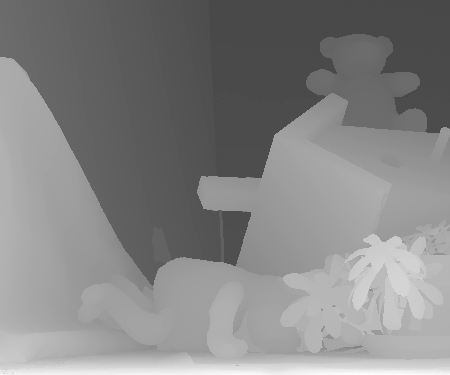
\includegraphics[width=0.9\textwidth]{results/rect.png}
        \caption{Square}
    \end{subfigure}
    \begin{subfigure}{.3\textwidth}
        \centering
        
\includegraphics[width=0.9\textwidth]{results/diamond.png}
        \caption{Diamond}
    \end{subfigure}
    \begin{subfigure}{.3\textwidth}
        \centering
        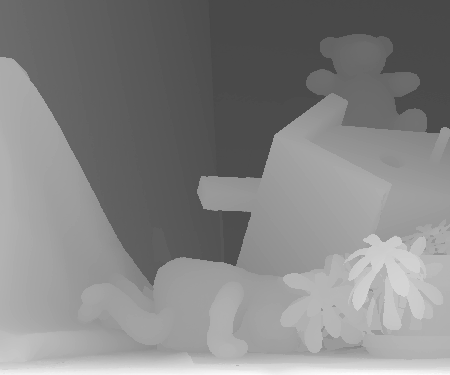
\includegraphics[width=0.9\textwidth]{results/plus.png}
        \caption{Cross}
    \end{subfigure}
    \caption{The result from different kernels}
    \label{fig:result_of_kernels}
\end{figure}

接著我們比較了不同 dilation 次數的影響,結果如 Figure \ref{fig:result_of_dilation_test}。我們分別做了1、5、9次的 dilation ,除了運算的時間增加以外,從結果來看幾乎看不出差異,因此之後的實驗統一使用 1 次 dilation。

\begin{figure}[h]
\centering
    \begin{subfigure}{.3\textwidth}
        \centering
        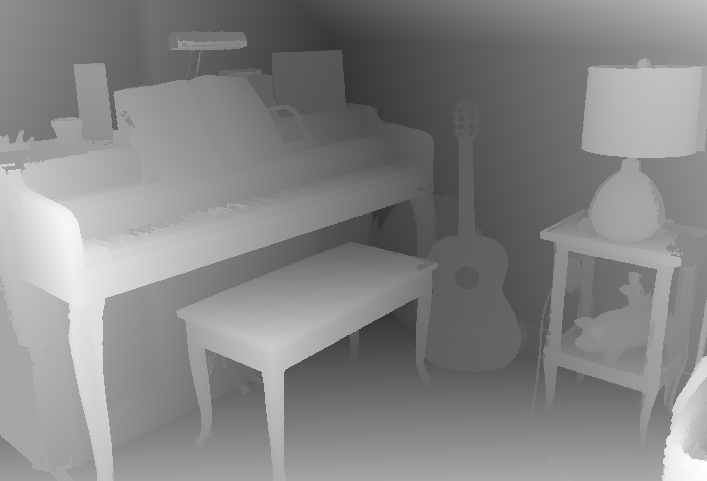
\includegraphics[width=0.9\textwidth]{results/dliate_1.png}
        \caption{with 1 dilation}
    \end{subfigure}
    \begin{subfigure}{.3\textwidth}
        \centering
        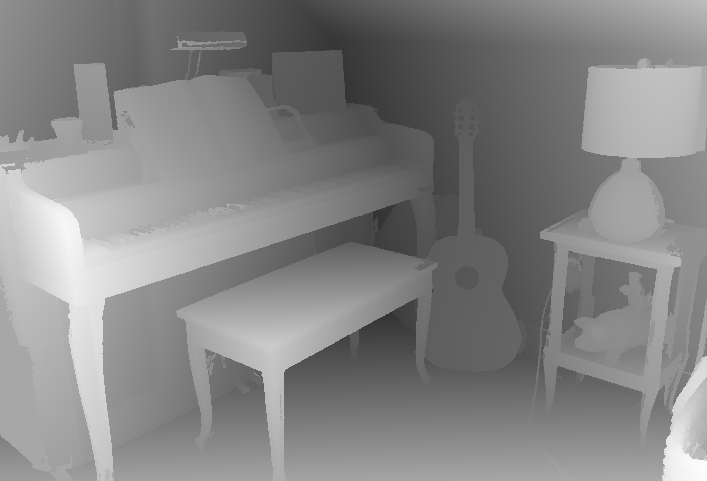
\includegraphics[width=0.9\textwidth]{results/dliate_5.png}
        \caption{with 5 dilation}
    \end{subfigure}
    \begin{subfigure}{.3\textwidth}
        \centering
        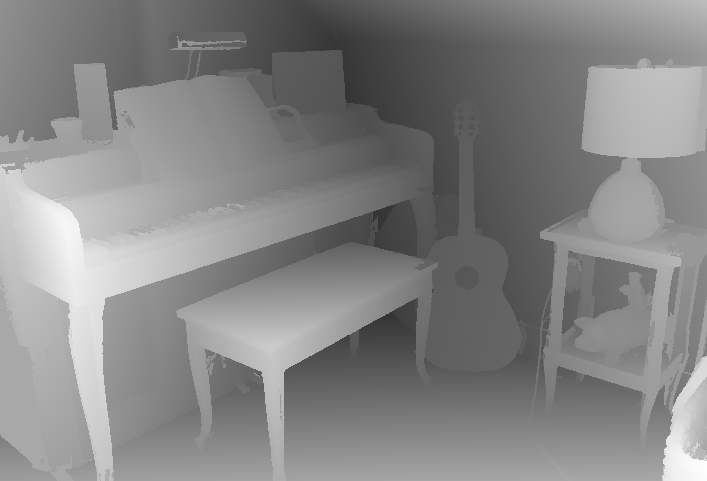
\includegraphics[width=0.9\textwidth]{results/dliate_9.png}
        \caption{with 9 dilation}
    \end{subfigure}
    \caption{The result of dilation tests}
    \label{fig:result_of_dilation_test}
\end{figure}

最後我們討論選值方法,首先把這些 pixels 用 histogram 做統計,第一種取值方法是用每個 pixel 的機率乘上 pixel value 求出期望值,用期望值當成是填補的數值;另一種是直接找出機率最高的 pixel value 當成是填補的數值,比較的結果如 Figure \ref{fig:result_of_filling_value_test}。由結果可以發現,直接選用機率最高的 pixel value 來填補的效果不甚理想,可以看到圖中白色架子會直接延伸到後方的平台上。反之,用期望值來填補的效果非常好,因此我們最後選用期望值來當成是我們填補的基準。

\begin{figure}[h]
\centering
    \begin{subfigure}{.45\textwidth}
        \centering
        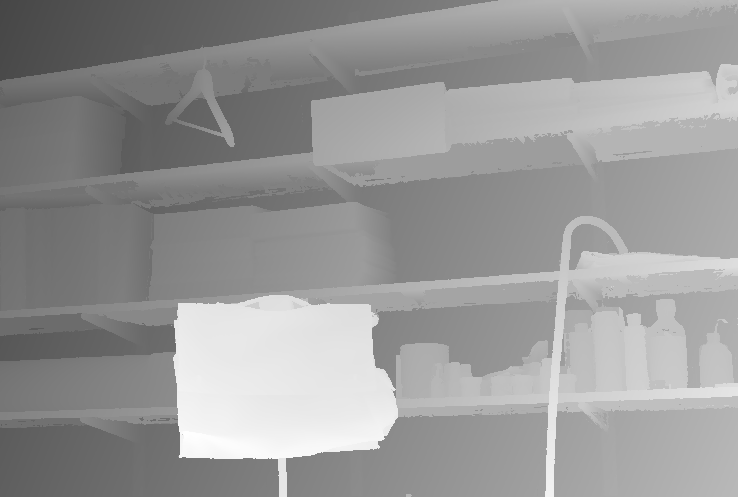
\includegraphics[width=0.9\textwidth]{results/mean.png}
        \caption{Mean value}
    \end{subfigure}
    \begin{subfigure}{.45\textwidth}
        \centering
        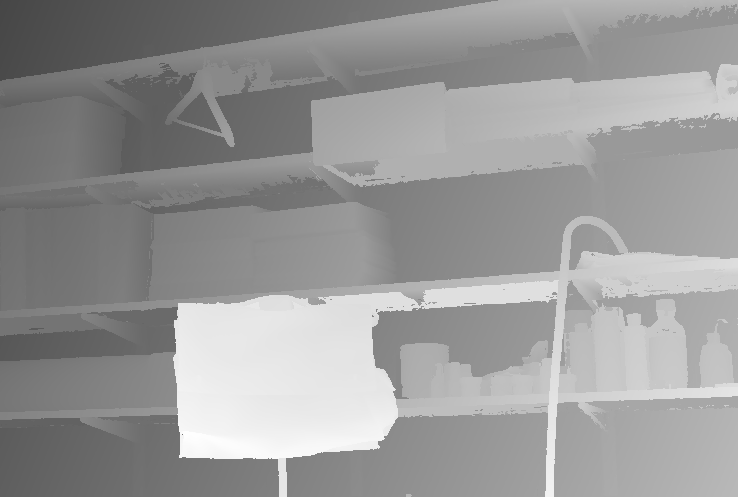
\includegraphics[width=0.9\textwidth]{results/max.png}
        \caption{Max value}
    \end{subfigure}
    \caption{The result of different approaches of choosing repair value}
    \label{fig:result_of_filling_value_test}
\end{figure}

\section{Conclusion}
我們花了很多時間利用python在重現四篇paper的方法(LR、LRTV、LRL0、{$\mathrm{LRL0^{\psi}}$}),跟paper結果進行比較,並理解了許多的專有名詞以及原理。並且發現使用這些方法的不足之處,所以我們利用了在本堂課程所學,利用dilation與histogram統計的方式優化paper所使用的方法,讓最後呈現的image inpainting不會有任何的缺失值,解決了{$\mathrm{LRL0^{\psi}}$}在遇到比較大的hole會比較劣勢的問題,而且運算速度極快,平均一張圖僅需要400ms的處理時間。雖然我們最終實作方法的PSNR結果沒有像paper所提到的那麼好,但是在視覺上的呈現結果卻比paper好了許多,在image inpainting上達到了非常完美的結果。

%\medskip


%%%%%%% Reference


\small
\bibliographystyle{ieeetr}
\bibliography{egbib}

\end{CJK*}
\end{document}
